\lstinputlisting[language=bash,basicstyle=\small]{python_codes/fieldstone_31/keywords.ascii}

\begin{center}
Code at \url{https://github.com/cedrict/fieldstone/tree/master/python_codes/fieldstone_31}
\end{center}

\par\noindent\rule{\textwidth}{0.4pt}
%%%%%%%%%%%%%%%%%%%%%%%%%%%%%%%%%%%%%%%%%%%%%%%%%%%%%%%%%%%%%%%%%%%%%%%%%%%%%%%%%%%%%%%%%%%%


We shall use here several 3D velcoity fields:

\begin{itemize}

%-----------------------------------------------------------------
\item vfield=1:

\begin{equation}
\vec{\upnu}
=
\left(
\begin{array}{c}
(y+z)(1-x^2) \\
(-x+z)(1-y^2) \\
(-x-y)(1-z^2) 
\end{array}
\right)
\end{equation}
Let us compute all the strain rate tensor components:
\begin{eqnarray}
\dot{\epsilon}_{xx}&=& -2x(y+z)  \nonumber\\
\dot{\epsilon}_{yy}&=& -2y(-x+z) \nonumber\\
\dot{\epsilon}_{zz}&=& -2z(-x-y) \nonumber\\
\dot{\epsilon}_{xy}&=& \frac{1}{2}(y^2-x^2) \nonumber\\ 
\dot{\epsilon}_{xz}&=& \frac{1}{2}(z^2-x^2)  \nonumber\\
\dot{\epsilon}_{yz}&=& \frac{1}{2}(y^2-y^2)  \nonumber
\end{eqnarray}
One can easily verify that $\dot{\epsilon}_{xx} +\dot{\epsilon}_{yy} +\dot{\epsilon}_{zz}=0$.

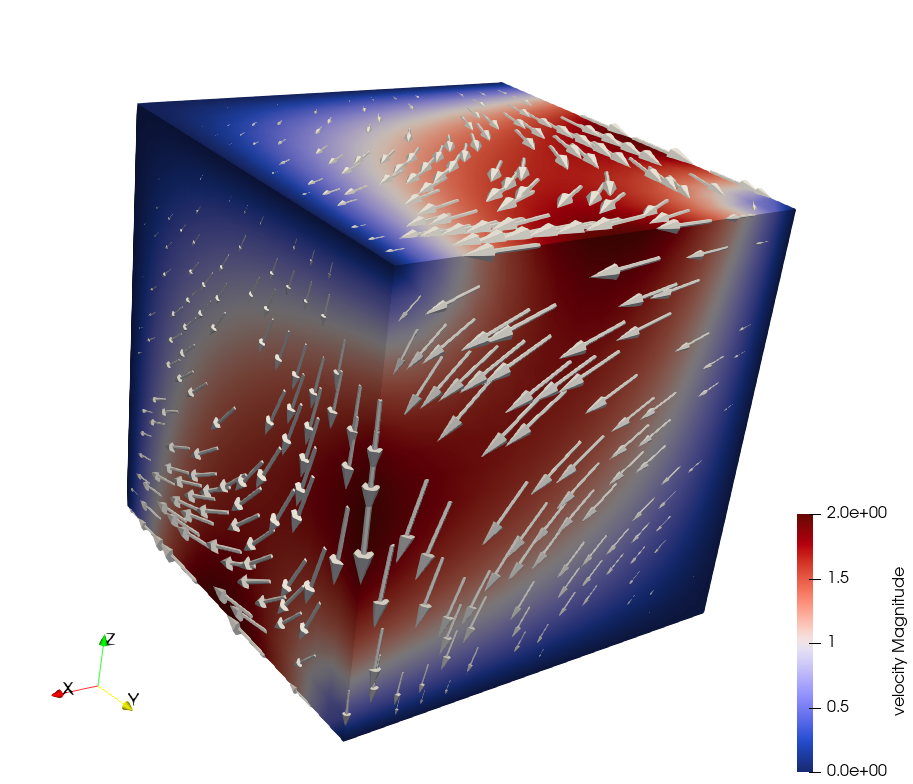
\includegraphics[width=4cm]{python_codes/fieldstone_31/velfield1}

%-----------------------------------------------------------------
\item vfield=2

\begin{equation}
\vec{\upnu}
=
\left(
\begin{array}{c}
(2-x^2-x^4)*(3*y+3*y^3)*(z+2*z*3)\\
(2-y^2-y^4)*(x+2*x^3)*(-z-2*z^3)\\
(2-z^2-z^4)*(-x-2*x^3)*(2*y+y^3)
\end{array}
\right)
\end{equation}

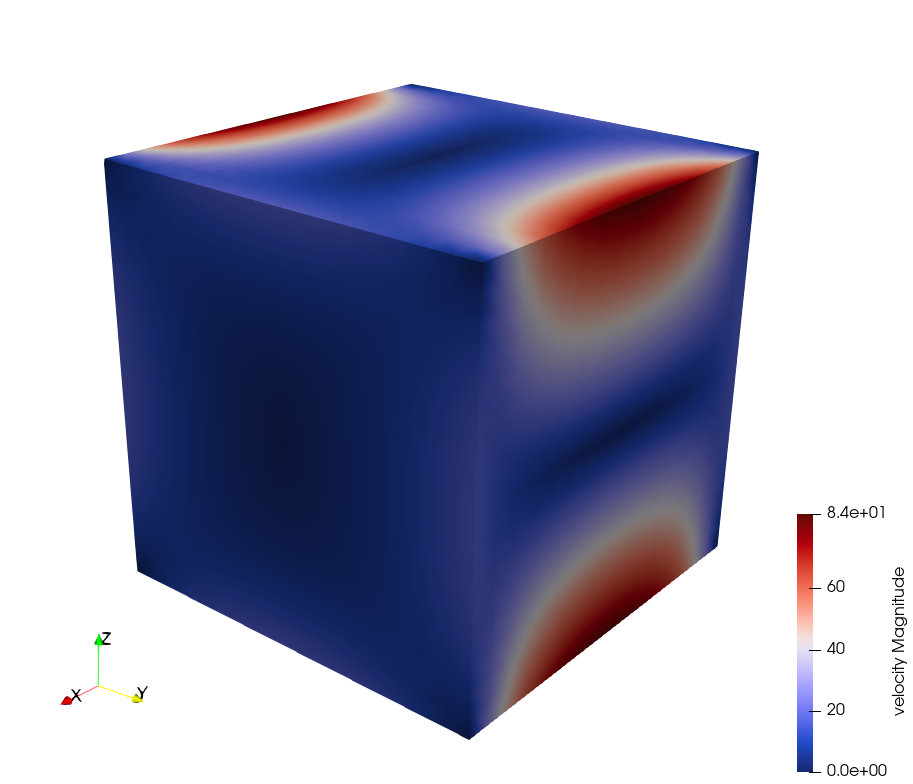
\includegraphics[width=4cm]{python_codes/fieldstone_31/velfield2}

%-----------------------------------------------------------------
\item vfield=3:

\begin{equation}
\vec{\upnu}
=
\left(
\begin{array}{c}
2*\sin(\pi*x)*\cos(\pi*y)*\cos(\pi*z)\\
-\sin(\pi*y)*\cos(\pi*x)*\cos(\pi*z)\\
-\sin(\pi*z)*\cos(\pi*x)*\cos(\pi*y)
\end{array}
\right)
\end{equation}

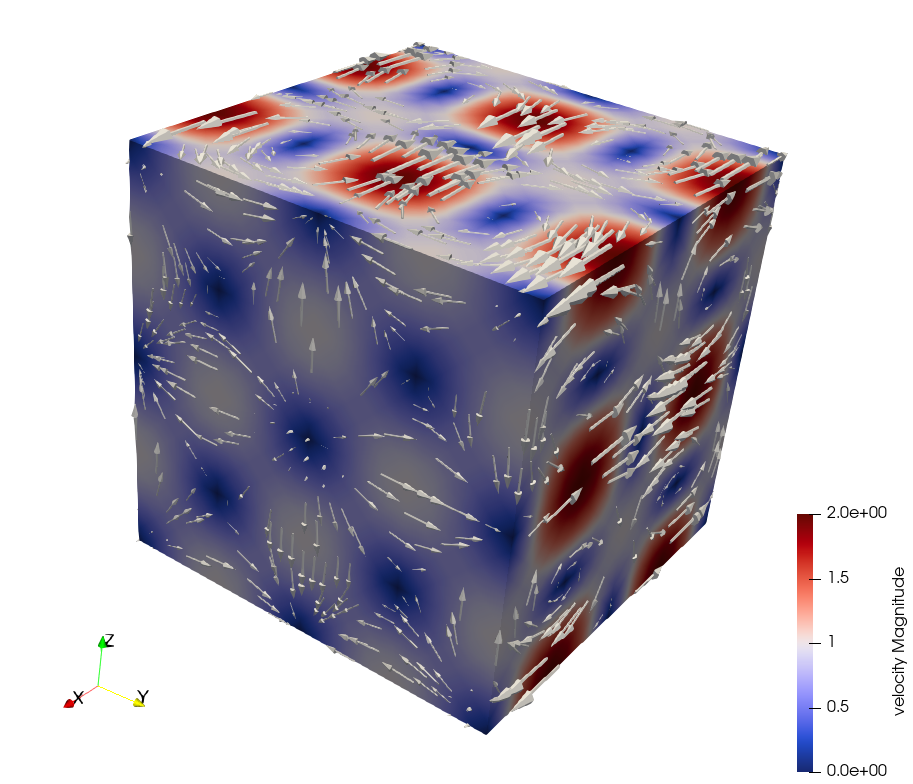
\includegraphics[width=4cm]{python_codes/fieldstone_31/velfield3}

%-----------------------------------------------------------------
\item vfield=4 (from \textcite{brtf08} (2008)):

\begin{equation}
\vec{\upnu}
=
\left(
\begin{array}{c}
\frac12 \sin(2\pi x) \cos(4\pi y) \cos(\pi z) + \sin(\pi x) \cos(2\pi y) \cos(\pi z) \\ \\
\frac14 \cos(2\pi x) \sin(4\pi y) \cos(\pi z) + \frac12 \cos(\pi x) \sin(2 \pi y) \cos(\pi z) \\ \\
-2\cos(2\pi x)\cos(4\pi y) \sin(\pi z) - 2\cos(\pi x)\cos(2\pi y) \sin(\pi z)
\end{array}
\right)
\end{equation}

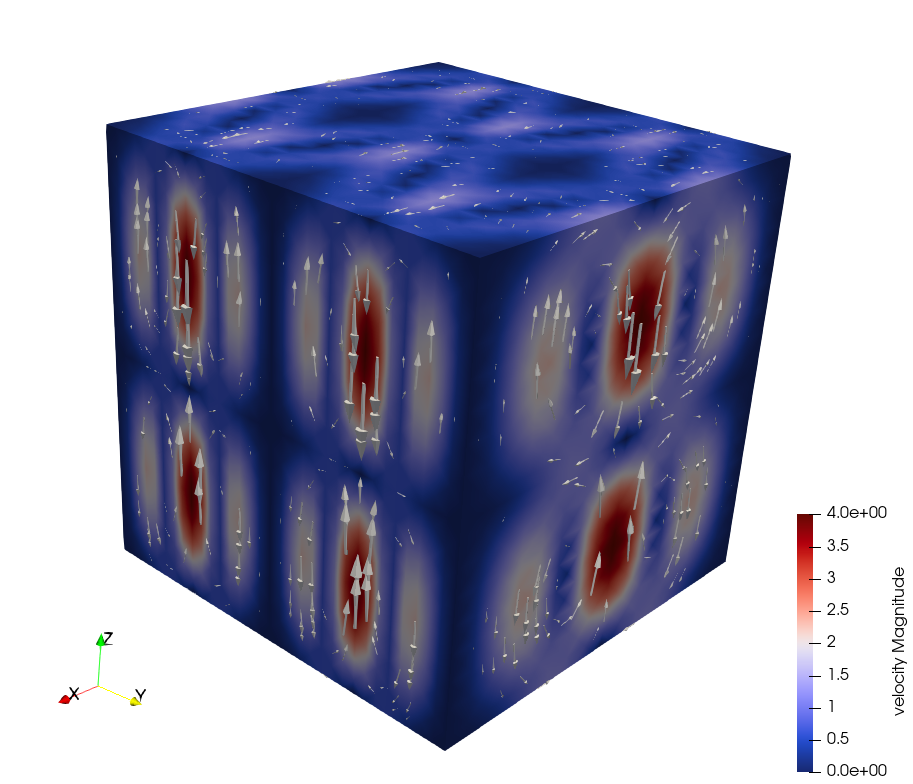
\includegraphics[width=4cm]{python_codes/fieldstone_31/velfield4}

\end{itemize}




TODO:

- implement all strain rate terms for all velocity fields

- make script  

- 


